\documentclass[twocolumn, 11pt, a4j]{article}

% The following packages can be found on http:\\www.ctan.org
\usepackage{graphics} % for pdf, bitmapped graphics files
\usepackage[dvipdfmx]{graphicx}
\usepackage[dvipdfmx]{color}
\usepackage{epsfig} % for postscript graphics files
\usepackage{mathptmx} % assumes new font selection scheme installed
\usepackage{times} % assumes new font selection scheme installed
\usepackage{amsmath} % assumes amsmath package installed
\usepackage{amssymb}  % assumes amsmath package installed
\usepackage{multicol}
\usepackage{multirow}
\usepackage{url}
\usepackage{caption}
\usepackage[ruled,vlined]{algorithm2e}

\usepackage[margin=15mm]{geometry} % マージン最小化
%\setlength\parindent{0pt}
\renewcommand{\baselinestretch}{0.8} % 行間スペース
\captionsetup[figure]{format=plain, labelformat=simple, labelsep=period, font=footnotesize}
\captionsetup[table]{format=plain, labelformat=simple, labelsep=period, font=footnotesize}

\usepackage[dvipsnames]{xcolor}
\usepackage{cite}

\setlength\textfloatsep{5pt}

\begin{document}
\twocolumn[
\begin{center}
  {\LARGE \bf{信頼される自動運転用LiDARに向けて~高解像度化とセキュリティ~}} \\
  \vspace{0.25cm}
  {\LARGE \textrm{吉岡 健太郎}} \\
  \vspace{0.2cm}
  {\textrm{慶應義塾大学(〒223-8522 神奈川県横浜市港北区3-14-1)}} \\
  \vspace{0.25cm}
  {\LARGE \bf{Towards Reliable LiDARs for Autonomous Driving: A Review of High-resolution and Security Features}} \\
  \vspace{0.25cm}
  {\LARGE \textrm{Kentaro Yoshioka}} \\
  {\textrm{Keio University}} \\
\end{center}

%%%%%%%%%%%%%%%%%%%%%%%%%%%%%%%%%%%%%%%%%%%%%%%%%%%%%%%%%%%%%%%%%%%%%%%%%%%%%%%%
\begin{abstract}
 信頼されるAIを実現するにはAI自身の習熟度以外にもセンサの"信頼性"が求められる。本講演では自動運転やロボティクスで必需3DセンサであるLiDAR(Light Detection and Ranging)の信頼性を主に高解像度化とセキュリティの二面から問う。まず3D情報を活用したAIが十分な信ぴょう性を持つためにはLiDARの高解像度が不可避である。そのような高解像度LiDARの実現方法を回路システム的見地から議論し、先端LiDARの発展と照らし合わせる。そしてLiDARのハッキング可能性について議論し、セキュリティ方面の研究を紹介し、最後にハッキングの防衛方法を講じる。

\end{abstract}
\vspace{0.5cm}
]
%%%%%%%%%%%%%%%%%%%%%%%%%%%%%%%%%%%%%%%%%%%%%%%%%%%%%%%%%%%%%%%%%%%%%%%%%%%%%%%%
\section{イントロダクション}
 人間は最新のハードウェアと比べても優秀なセンサや判断機構を持つ一方で時に信じられないほど幼稚なミスを犯してしまう。そしてそのようなミスは自動車の運転時に取り返しのつかない結果をもたらす。日本のみでも2021年における交通事故死亡者数は2,636人であり負傷者数は361,768人に登る\cite{keisatsu}。このようなミスをゼロにするのは不可能であるため、人間のミスをカバーするためにAdvanced Driver-Assistance Systems(ADAS)技術が発展してきた。SAEでは自動運転にはレベルが5つ設定されている\cite{sae}。例えば2022年現在、自動ブレーキやレーンキーピングといったレベル0-1の自動運転は多くの市販車に搭載されている。またTesla社はレベル2の部分自動運転機能をリリースしており、国内メーカでも速度や使用箇所に限定はあるもののレベル3相当の自動運転機能を搭載した製品もある。このように時間をかけ人間ドライバーから機械制御へ運転機能を任せようとしている。

ADASに使用するDepthセンサについてまとめた表がTable \ref{sensor}である。重要なことはいずれのセンサも性能にトレードオフが存在することである。
自動運転用LiDARはミリ波レーダ、ステレオカメラ、超音波と異なりスキャンを行う機械部が必要となり、他のセンサに比べコストが高くなる。一方でLiDARは距離センサの中でも高い解像度が得られる唯一の距離センサであることから注目を集めている。

自動運転用距離センサに求められる遠距離性能と画像分解能についてより詳しく触れる。一般的に自動運転の前方監視には120km/hで高速道路にて走行する際のブレーキ距離が150mであることから、前方200mをセンシングする距離センサが求められる。例えば自動運転のプロトタイプ車で採用されているVLP-32\cite{velodyne, velopatent}は最大距離は50mと短く高速道路利用の要件は満たさない。また市街地を走行する際には遠方の歩行者を見落とさないのが重要な要件である。これには0.1~0.2度の水平角度分解能が求められ超音波やレーダ\cite{mitomo201077}で達成するのは非常に難しい。
また自動運転の信頼性を高めるためにはあらゆる天候(非常に強い日差し、雨、雪、霧)でセンシング可能であることは重要である。中でもミリ波レーダは天候の影響を受けづらいセンサであることが知られている。反面LiDARは例えば霧といった環境に置かれるとレーザが散乱するため有効距離が短くなってしまう。そのため一つのセンサで自動運転システムを構築するのは難しく、最終的にはセンサ同士がお互いの弱点をかばい合うセンサフュージョンアプローチを取る必要がある。

本論文の対象読者はこれから車載LiDARについて入門するレベルを想定しており、車載LiDAR分野の発展方向を俯瞰し捉えることを目標とする。メインにカバーするのは2022年現在最も車載用途で量産化が期待される850-950nmの遠赤外レーザを用いるスキャン機構を持つdToF型LiDARである\cite{niclass2012100, yoshioka201820, kondo2020automotive, ta20202d, kumagai2021189x600}。
本論文の構成は以下である。まず2章ではLiDARの原理から車載LiDAR特有の課題について説明する。そして3章ではベースとなる第一世代LiDARから次世代LiDARへの発展をカバーする。
そして4章ではLiDARのセンサセキュリティについて述べる。
最後に5章でまとめと今後の展望を述べる。

\begin{table}[!t]
\centering
\caption{車載距離センサの特性.LiDARは分解能や距離といったバランスに優れるが長年コストが課題となっていたが、近年集積回路化によってLiDARの低コスト化が進んでいる。}
 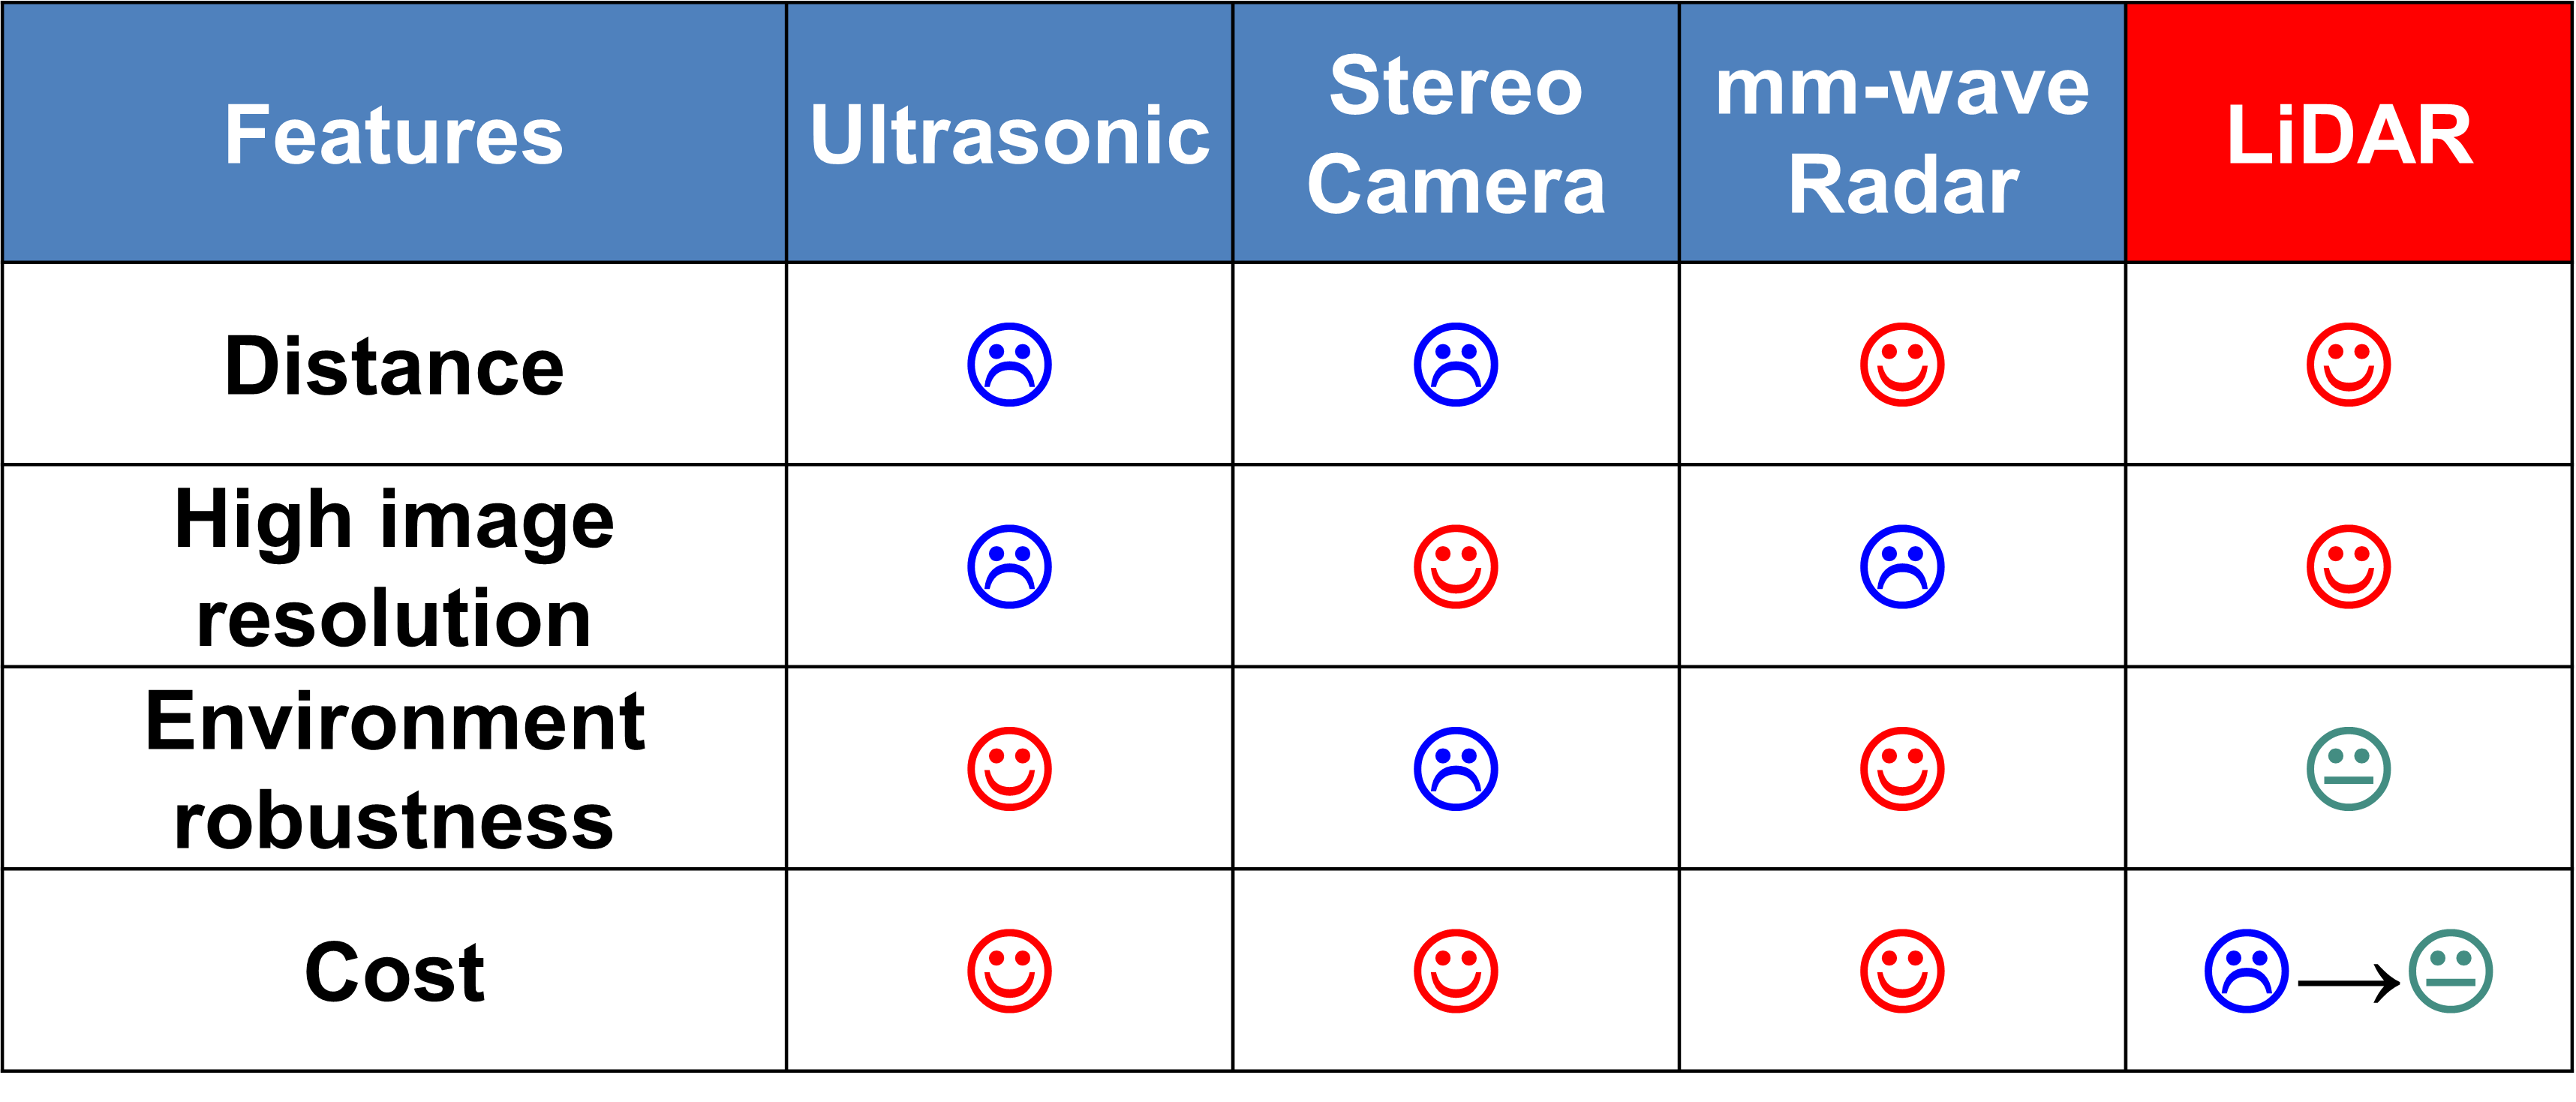
\includegraphics[width=0.4\textwidth]{figs/distancesensor.png}
\label{sensor}
\end{table}

%%%%%%%%%%%%%%%%%%%%%%%%%%%%%%%%%%%%%%%%%%%%%%%%%%%%%%%%%%%%%
\section{LiDAR原理と車載特有の課題}
\begin{figure}[!t]
\centering
 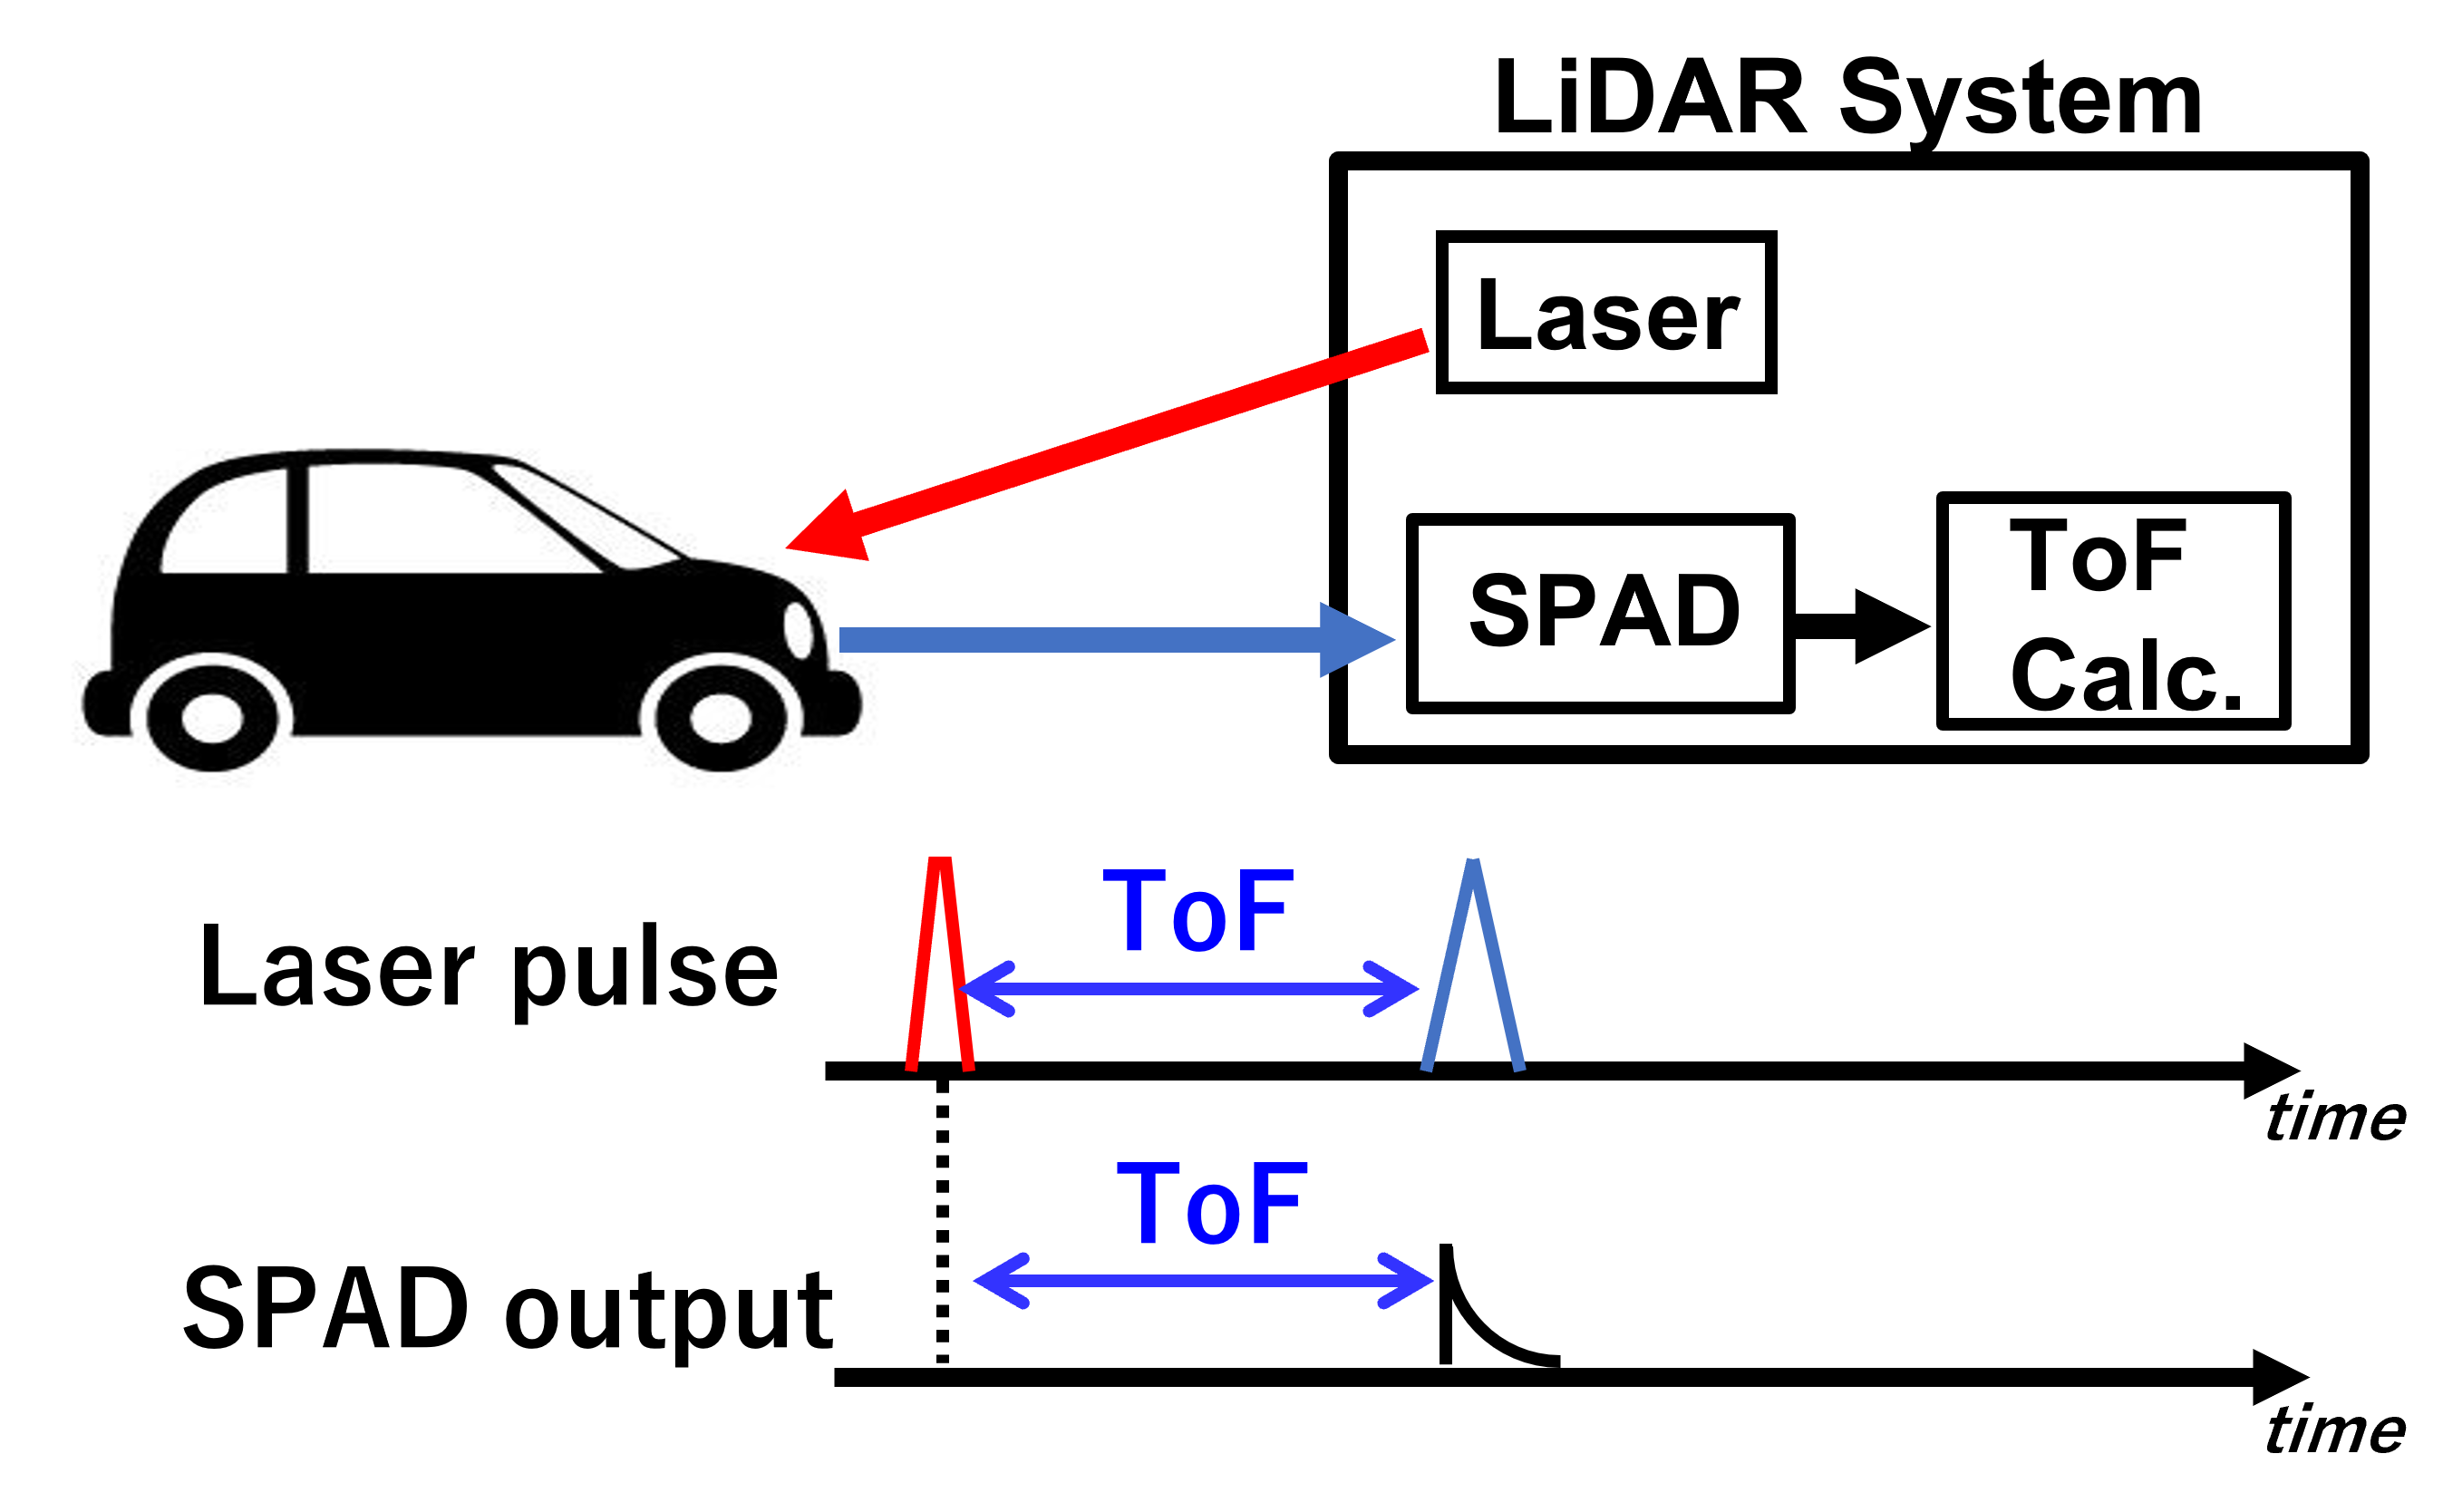
\includegraphics[width=0.4\textwidth]{figs/lidar.png}
  \caption{lidar measurement}
\label{lidar}
\end{figure}

\begin{figure}[!t]
\centering
 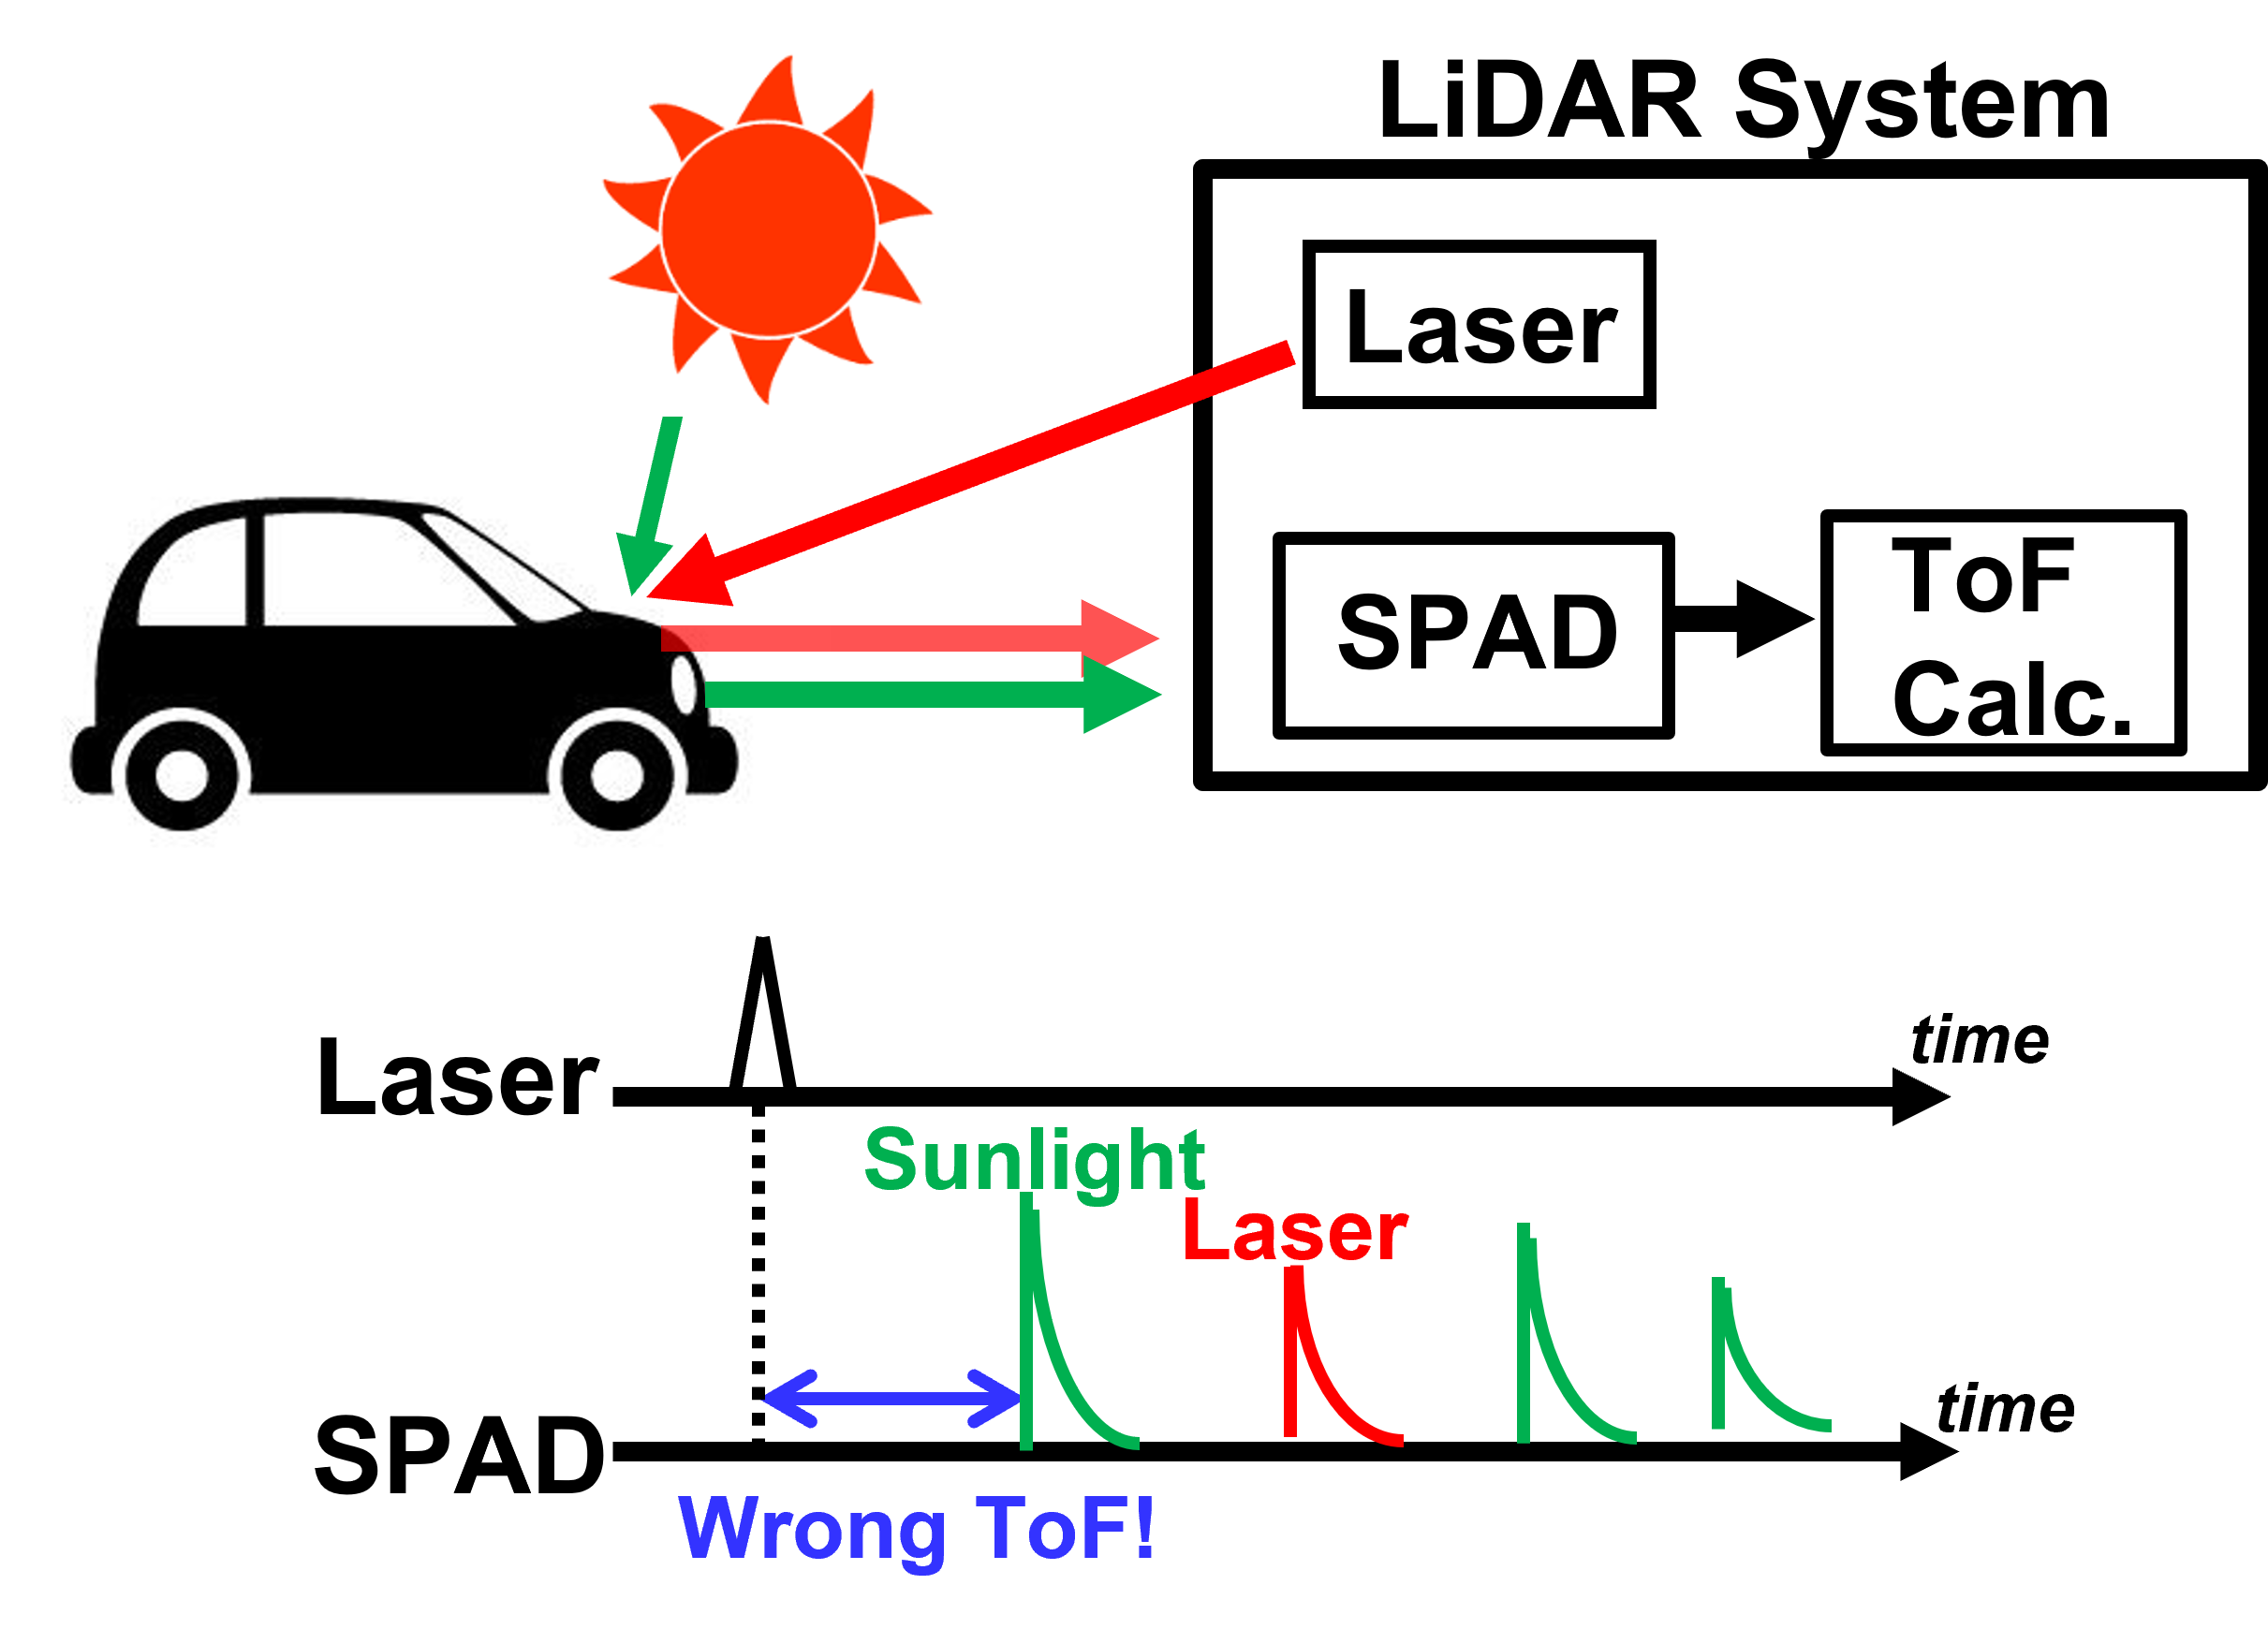
\includegraphics[width=0.4\textwidth]{figs/sunlight.png}
  \caption{sunlight lidar}
\label{sunlight}
\end{figure}

 本論文で取り扱うdirect Time of Flight(dToF) LiDARの動作原理をFig.\ref{lidar}を元に簡単に説明する。このようなLiDARは筐体から出射したレーザが対象物体に反射し戻ってくるまでの時間(time-of-flight ToF)を元に
\begin{eqnarray}
    \centering
    \textrm{Distance} = \frac{\textrm{Light speed} \times \textrm{ToF}}{2}
    \label{dist}
\end{eqnarray}
と距離を導出する。精度の高い(距離分解能の高い)計測のためにLiDARが備える量子化器の時間分解能は高速である必要がある(ADCならばサンプルレートが高い等)。

LiDARの原理自体は単純なものの、車載用LiDARは主に以下の点で設計が難しい:
\begin{itemize}
\item 高速で移動する車体に取り付けられるため、遠距離測距性能が要求される
\item 様々な天候・環境で高精度な計測が期待される。
\end{itemize}
前者に関してだが、レーザは距離の自乗に従い減衰するため、例えば50m測距に比べると200m測距では帰還するレーザ光子数は1/16となってまい動作はとても厳しい。また野外で使用するLiDARでは太陽光が最大のノイズ源となり、特に車載用途では100kluxといった非常に強い太陽光下でも動作することが要求される。このような過酷な動作環境をFig.\ref{sunlight}に示しており、遠距離かつ強い太陽光の環境下ではレーザよりも太陽光のパルスが大きくなる事もあり測距は非常に難しい。

LiDARの測距は原理的にはSNRで表現できる。ここでsignalは帰還するレーザ光子数、ノイズはある単位時間に入力されるノイズ光子数と定義して表せる\cite{yoshioka201820}。
\begin{eqnarray}
    \centering
    \textrm{LiDAR SNR} = \log_{20}{\frac{\textrm{Number of laser photons}}{\textrm{Number of background photons}}}
    \label{snr}
\end{eqnarray}
ここで車載LiDARのもう一つの制約として出射レーザパワーはeye-safetyを守らなければならない。車載用であれば最も厳しいclass-1 eye-safety、つまりどんな状況でも人の目に害を与えないレーザであることを遵守するのが一般的である。つまり出射可能なレーザパワーには厳しい制限があり、既に各研究はそのリミットギリギリでレーザ設計を行っていることを念頭に置く必要がある。一方でeq.\ref{snr}より太陽光をフィルタリングする光学フィルタやレーザ受光光子数を増やす受光素子の感度向上はSNRに寄与することがわかる。

\subsection{LiDARの基本アーキテクチャ}
\begin{figure}[!t]
\centering
 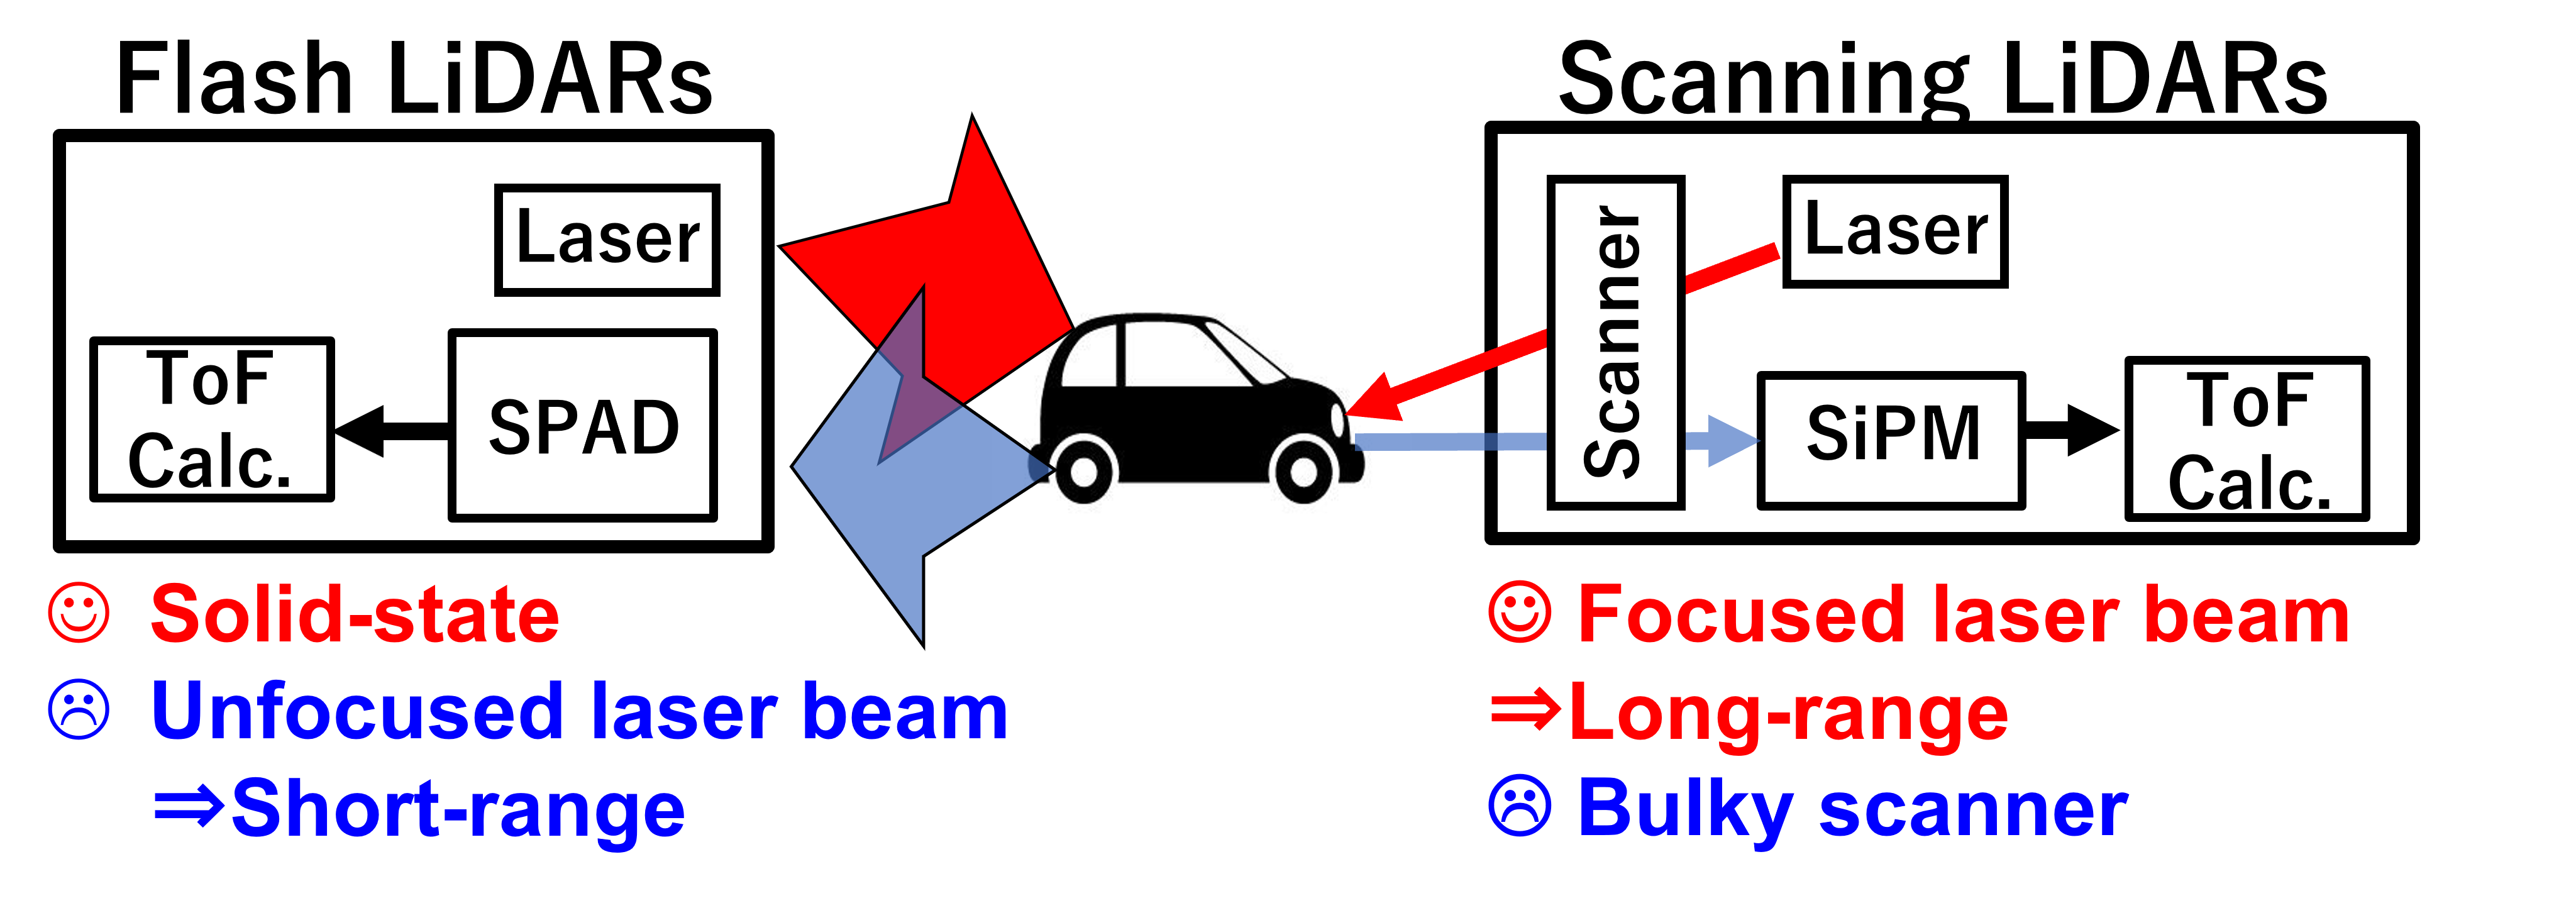
\includegraphics[width=0.49\textwidth]{figs/flashscan.png}
  \caption{flash or scan}
\label{flash}
\end{figure}

 Fig.\ref{lidar}に示す測定方式はdirect Time of Flight(dToF)方式と呼ばれ、車載LiDARで遠距離測定が可能な主流方式である。dToF型LiDARはその中でもフラッシュ型\cite{ximenes2018256}とスキャン型に大別される。Fig.\ref{flash}に示すとおり、フラッシュは画角全面にレーザを放射し反射光もイメージセンサのような2次元の受光素子アレーで受ける。この方式のメリットとして機械部がないため低コストで実現できるのに加え、フレームレートも早い。一方でFlash LiDARの画素数を$N\timesM$とすると、レーザ電力$P$は$N\timesM$画素に拡散されるため画素毎のレーザパワーは$P/(N\timesM)$と弱い。そのためFlash型では高解像度化は容易な反面、$>$100mといった遠距離測定を実現できている例は少ない。一方でスキャン型は一度に$M$ピクセルを得て水平、または二次元的にスキャンする。この方式のメリットとしてレーザを絞れるためピクセル毎のレーザパワーは$P/M$とフラッシュ型に対し非常に良好なSNRを達成可能で遠距離測定が実現できる反面、スキャン機構が必要なため製造コストが大きいというトレードオフを持つ。

スキャン方式にも回転ミラー\cite{velodyne,ouster}、ポリゴンミラー\cite{niclass2012100,yoshioka201820,kondo2020automotive}、MEMSミラー\cite{kumagai2021189x600}と複数種類が存在する。回転ミラーは筐体サイズは非常に大きいが光学特性がよく(レーザ減衰が少ない)、360度のデータが取得可能なことが特徴である。
ポリゴンミラーはFoV中をラスタースキャンすることでデータを得る。このようなスキャンを行うためにはレーザと受光両方に対しミラーを挿入する必要があり、ミラーを駆動するモータも合わせ筐体が大きくなってしまうのが欠点である(車載用途ではセンサ体積を最小化することが求められる)。
最後にMEMSミラーは可動ミラーをMEMSミラーを使い実現することでbulkyな機械部とモータをなくす。よってLiDAR筐体サイズをかなり小さくすることができる。MEMSミラーは可動部品であるものの、ポリゴンミラーや回転ミラーと区別するため慣習的にソリッドステート型LiDARとも呼ばれる。一方でMEMSミラーは小さく光学特性は劣悪なためLiDAR SNRが大きく低下するのがトレードオフである。

%%%%%%%%%%%%%%%%%%%%%%%%%%%%%%%%%%%%%%%%%%%%%%%%%%%%%%%%%%%%%%%%%%%%%%%%%%%%%%%%
\section{第一世代と次世代LiDAR}
\subsection{第一世代LiDAR}
\begin{figure}[!t]
\centering
 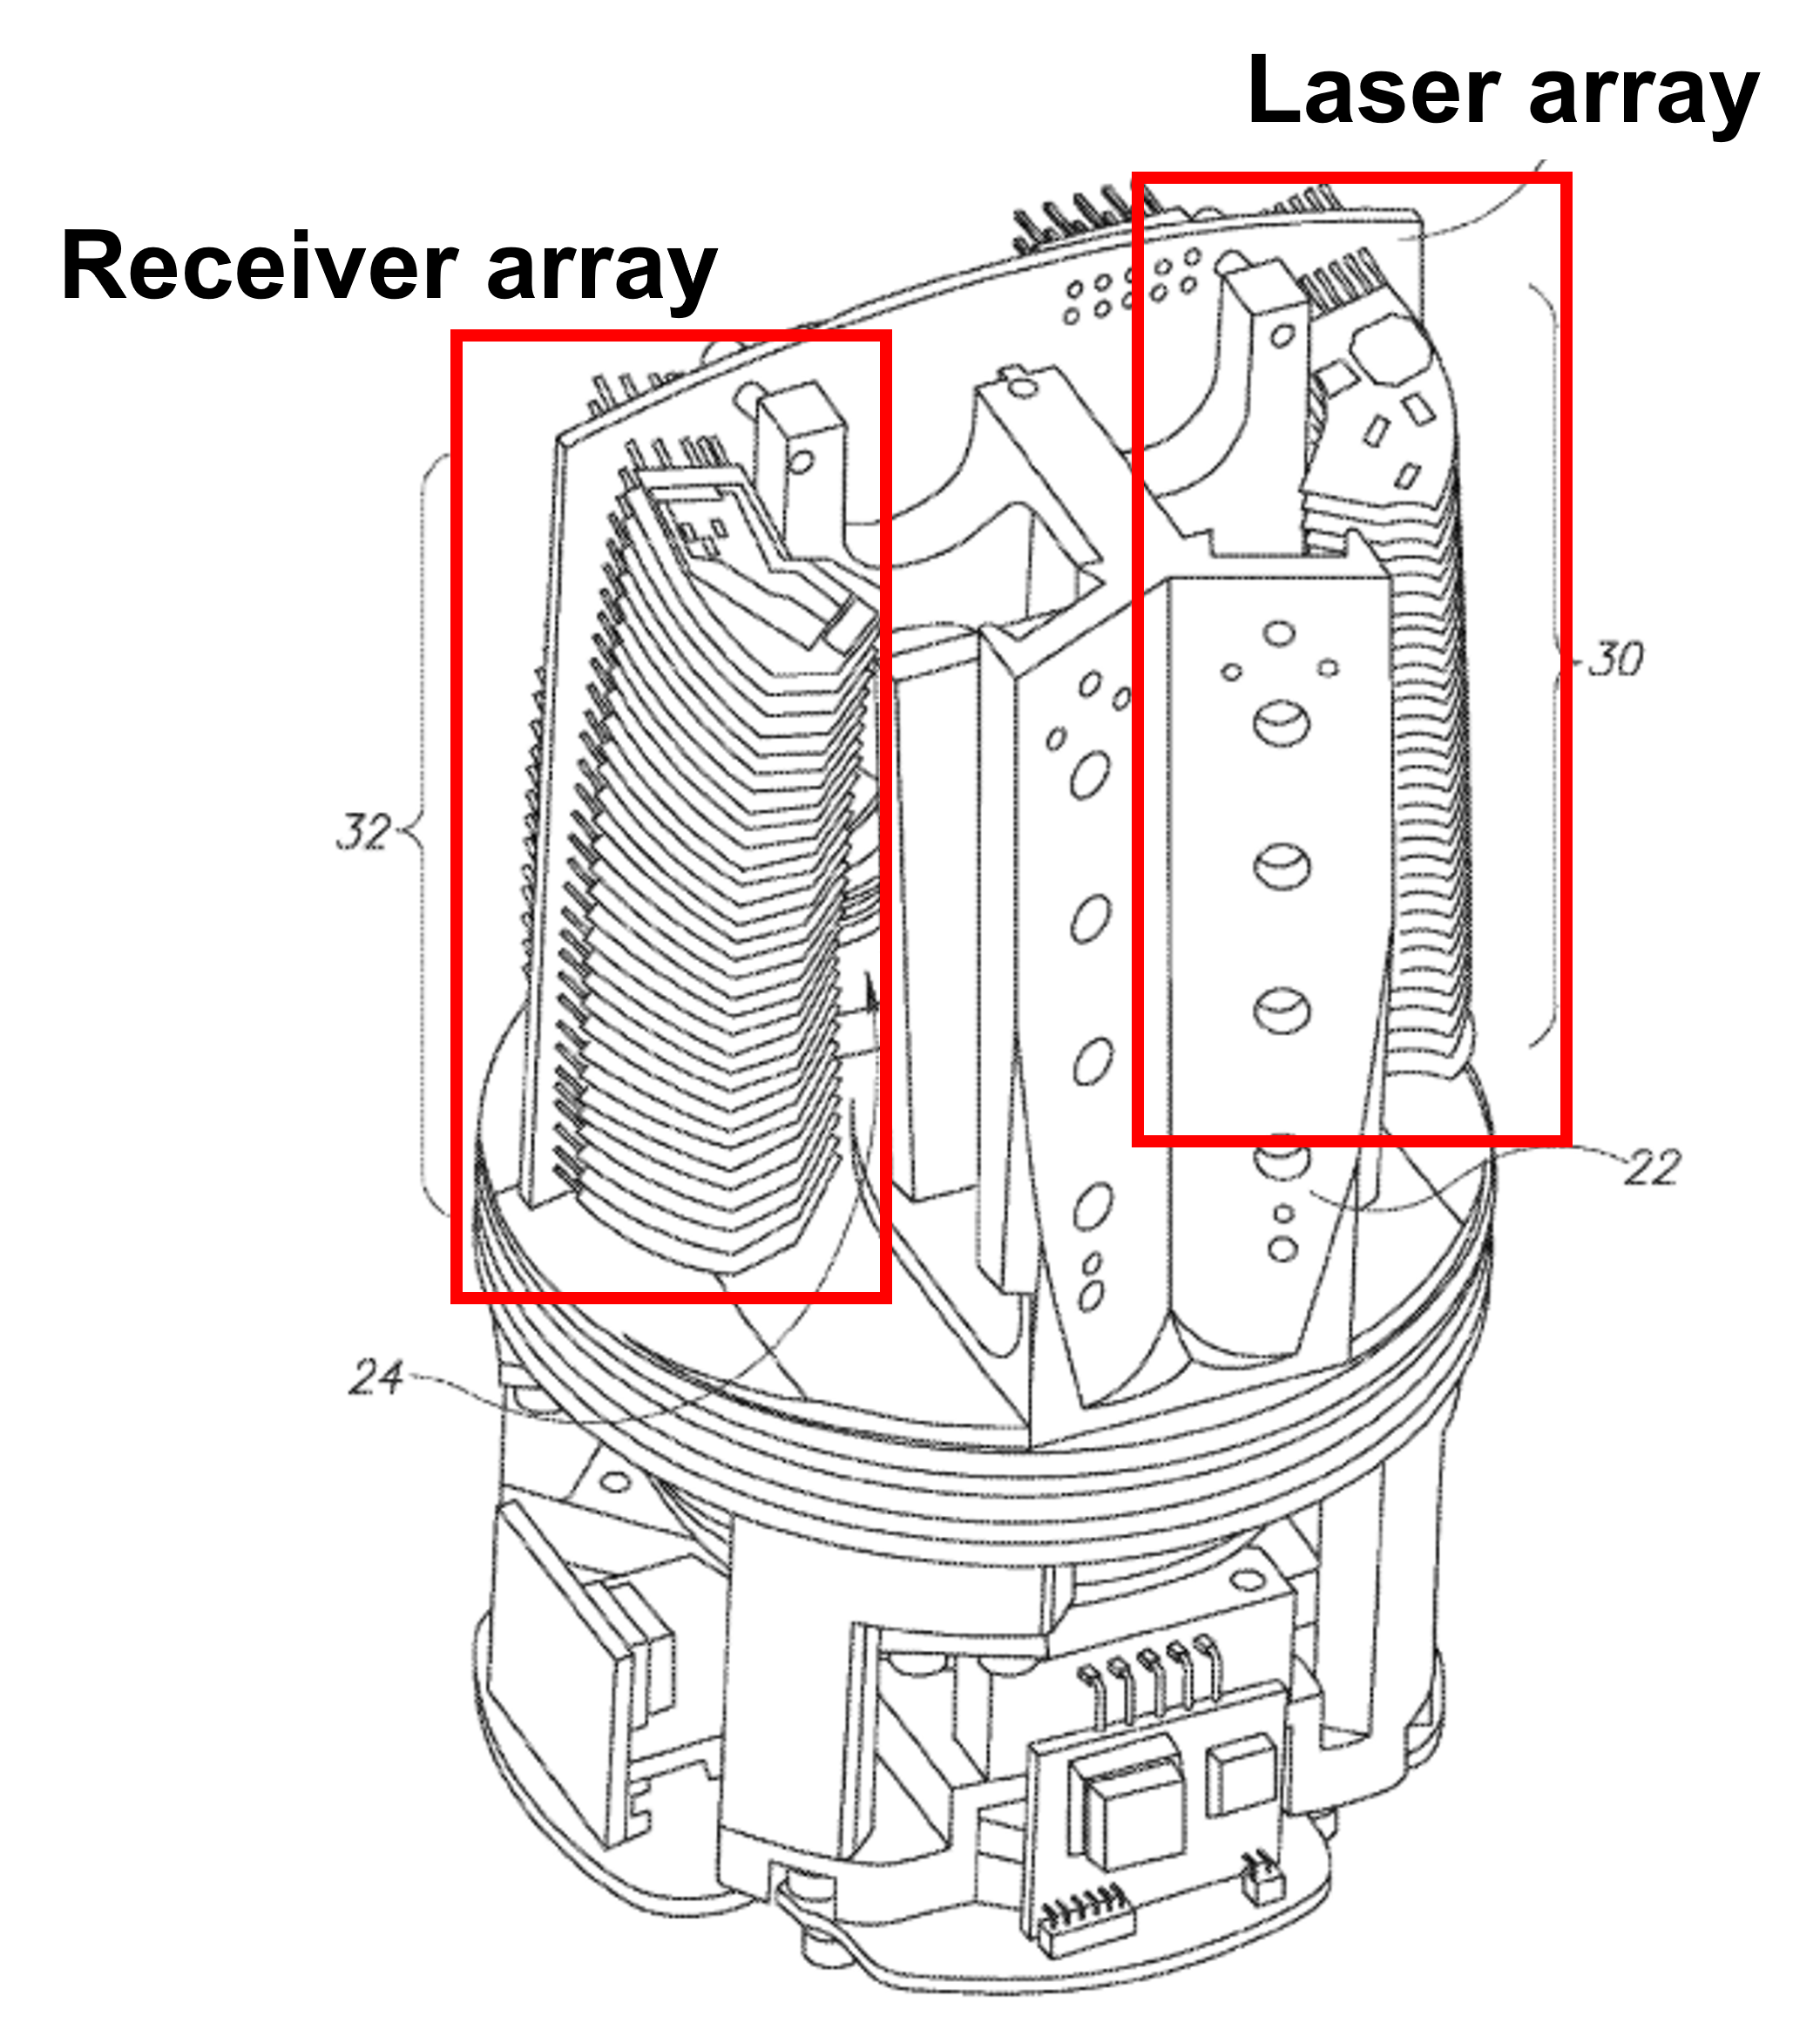
\includegraphics[width=0.34\textwidth]{figs/velo.png}
  \caption{Velodyne HDL-32 diagram \cite{velopatent}}
\label{velo}
\end{figure}

 Fig.\ref{velo}に示すVelodyne社の回転型LiDAR\cite{velodyne, velopatent}は縦方向にレーザと受信機のボードを積層することで実装されている。
これはLiDAR黎明期に出された製品であることから、第一世代LiDARと定義する\cite{yoshiokaieice}。このLiDARは非常に高品質な3Dセンシングを実現し多くの自動運転プロトタイプに使われた\cite{montemerlo2008junior}。

Fig.\ref{next}(a)に回路図を示すとおり、第一世代LIDARの受光素子にはAPDが使われ、APD出力をTIA及びVGAで増幅した後に高速ADCで量子化しToFを計算する。
\textbf{第一世代LIDARは各レーザと受光素子のペアで”点”の測定を行う距離センサ(2D LiDAR)をある種"力技"で多数実装することで、高解像度なLiDARを実現していると捉えることができる。}
一方でこのような実装には膨大な数の部品が必要である。結果として第一世代LiDARは非常に高価で壊れやすくなってしまった。加えて解像度を増やすには部品点数が更に増加してしまうため、同じ筐体で性能をスケールさせるのは難しい。またAPDは一般的なフォトディテクタよりは高感度であるものの、遠距離測定には不十分であった。第一世代LiDARの距離性能は最大50mと高速道路における要求を満たすのは難しかった。

%%%%%%%%%%%%%%%%%%%%%%%%%%%%%%%%%%%%%%%%%%%%%%%%%%%%%%%%%%%%%%%%%%%%%%%%%%%%%%%%
\subsection{次世代LiDAR}
\begin{figure*}[!t]
\centering
 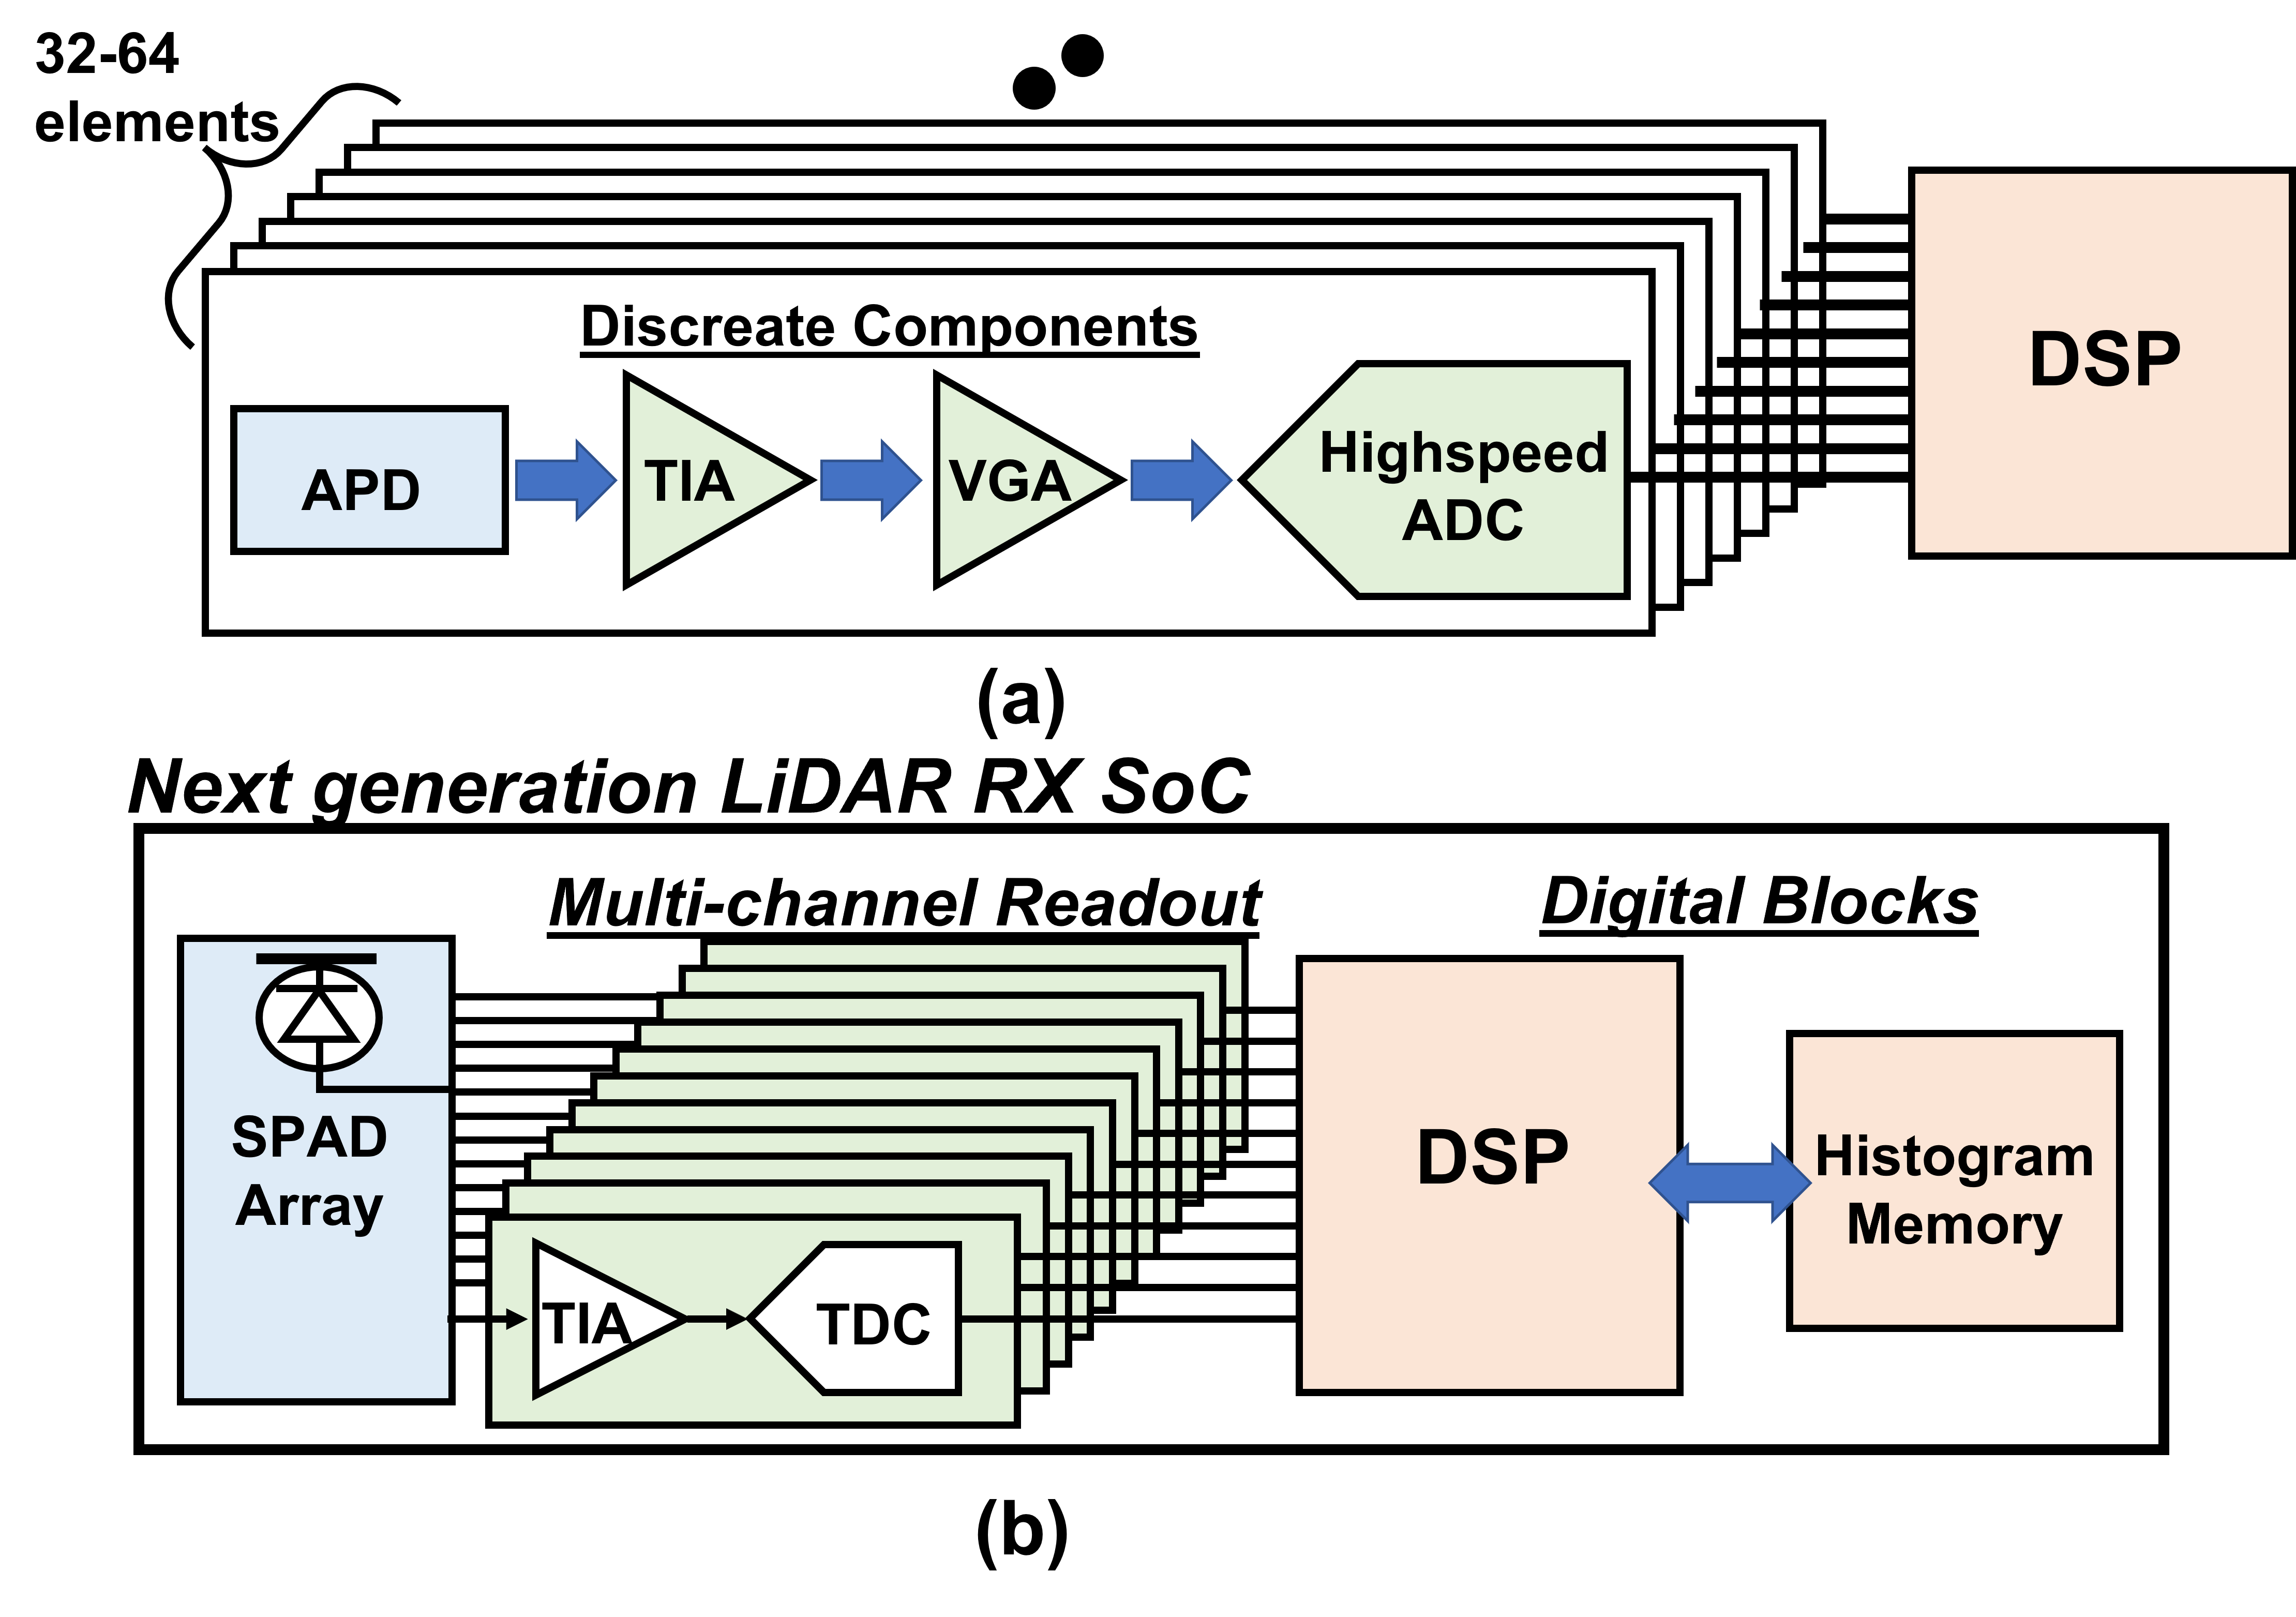
\includegraphics[width=0.7\textwidth]{figs/nextlidar.png}
  \caption{First-gen vs Next-gen lidars}
\label{next}
\end{figure*}

\begin{figure}[!t]
\centering
 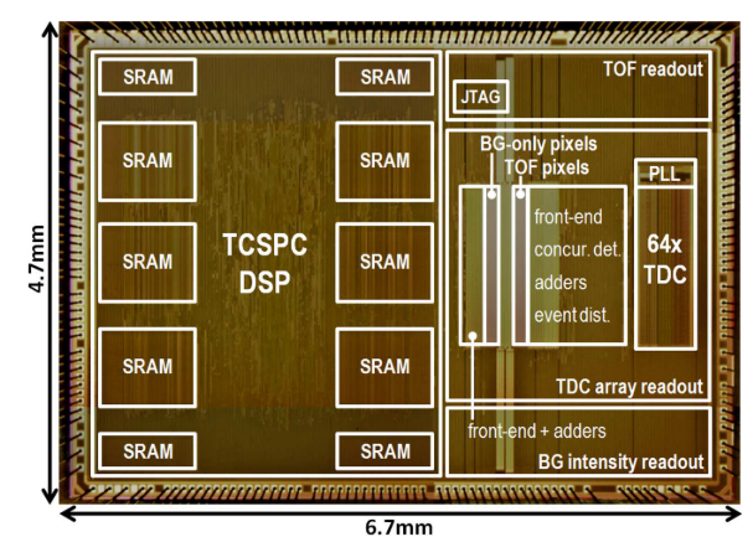
\includegraphics[width=0.4\textwidth]{figs/niclasschip.png}
  \caption{Fully integrated LiDAR SoC \cite{niclass2012100}}
\label{chip}
\end{figure}

 第一世代LiDARによって自動運転の研究や実証が進み、LiDAR市場は急拡大したものの、低コスト化に加えさらなる性能向上が進まなければ量産車への採用は難しい。このような目標を達成するため、次世代LiDARの研究が進められてきた。
本論文では次世代LiDARは\textbf{SPAD、読み出し回路、そして信号処理回路の集積化}によって実現されたと捉える。
第一世代と次世代LiDARを回路レベルで対比しているのがFig.\ref{next}である。

Ref.\cite{niclass2012100}ではSPADアレーと読み出し回路、DSP及びメモリをワンチップに集積した事でLiDARハードウェアにおけるブレイクスルーをもたらし、次世代LiDARへの道筋を立てた。車載LiDAR用では後述する通りクエンチング時間を緩和するために画素辺りのSPAD数は数10となり、結果としてSPADアレー全体の素子数は100-1000のオーダが必要となる。これらSPADアレーと信号処理回路をボード上で接続するのは実装上難しい。そこでref.\cite{niclass2012100}では高電圧を扱えるhigh voltage CMOSプロセスでSPADと読み出し回路、DSP、メモリをSystem on Chip(SoC)化し、ワンチップにLiDARに必要な部品のほとんどを集積した。
数多くのディスクリート部品を用いていた第一世代LiDARに対しワンチップで同じ機能を実現することで、圧倒的な低コスト化への道筋をつけた。またSoCではムーアの法則に則りCMOSスケーリングによって回路素子の性能向上を見込めるため、LiDAR性能もスケール可能となった。

\subsection{受光素子}
\begin{figure}[!t]
\centering
 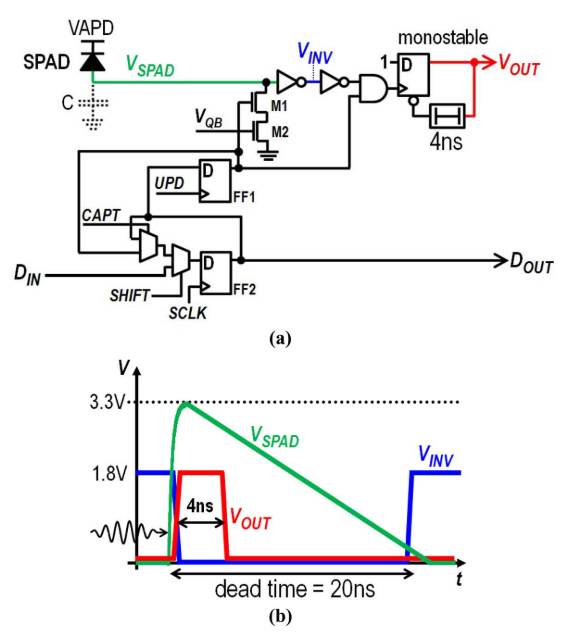
\includegraphics[width=0.4\textwidth]{figs/spad.png}
  \caption{SPAD \cite{niclass2012100}}
\label{spad}
\end{figure}

 APDもSPADもフォトダイオードを強い逆バイアスで動作させることは同じだが、SPADは非常に感度が高くシングルフォトン検出も可能な受光素子である\cite{niclass2005design}。SPADはブレイクダウン電圧+$\alpha$でバイアスすることでダイオードをガイガーモードで動作させる。ガイガーモードでは光子を受光すると理想的には素子の増幅率は無限大となり、光の強度に依存せず大電流を流すため単一光子の検出を可能とする。一方でこのような電流が流れ続けるとデバイスが破壊されてしまうため、付随したクエンチング抵抗によって負帰還をかけ強制的に電流を止める。

SPADはその強烈な増幅率によって光子一つの検出を可能とし微弱なレーザ光も検出できLiDARの遠距離性能に寄与する。キーパラメータは感度に直結する光子の受光確率である(photon detection efficiency (PDE))。もう一つはクエンチングを行ってから元のモードに戻るまでに掛かる時間(クエンチング時間)である。前者が高ければ高いほど微弱なレーザ光も検出できるため遠距離性能に直結する。また後者のクエンチング時間は太陽光耐性と密接に関係し、クエンチング時間が長いと太陽光といったノイズ光でSPADが発火した後にレーザ光に反応できないパイルアップが起きてしまう。クエンチング時間を低減するにはクエンチング抵抗を低下させるのが一番であるがデバイスの信頼性のトレードオフとなってしまう。%一般的には画素に複数SPADを配置しあるSPADが発火しても他SPADでレーザを受光する冗長性を組むことでパイルアップを緩和する。

\subsection{TDCベース読み出し回路}
 APDの出力は通常のPDと同じく光量に比例したアナログ量であるのに対し、SPADは無限の増幅率を持つため光子入射時の出力をバッファで整形することでデジタルパルスとして扱うことができる。出力がパルスであったとしてもdToF LiDARであればtime of flightを測ることができれば距離測定は可能である。またSoC上に数10,数100の高速ADCを実装するのは面積的に難しいが、\cite{niclass2012100}ではToFを測ることに特化した回路であるtime-to-digital converter (TDC)回路が使用されている。TDCはデジタルPLLの時間量子化回路として登場した回路であり、入力された時間差のデジタル値を得る回路である\cite{leetdc, elkholytdc}。
特徴としてTDCはADCに比べほぼデジタル回路のみで構成することができるため、少ない面積で大量のTDC回路を実現できる。加えてTDCの一般的な時間分解能は10-100psと高く、ADCでは実現できないToF精度を達成できるためLiDAR SoC化に好適である。

\subsection{信号処理回路}
\begin{figure}[!t]
\centering
 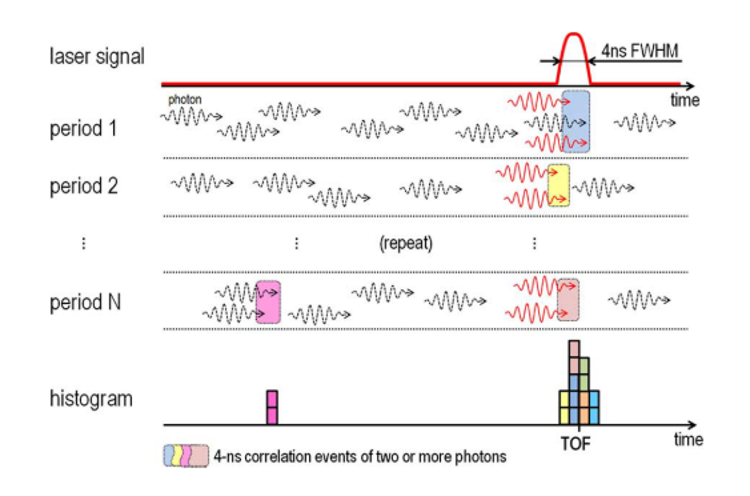
\includegraphics[width=0.5\textwidth]{figs/threshold.png}
  \caption{TDC readout \cite{niclass2012100}}
\label{tdc}
\end{figure}

 SoC化によってリッチな信号処理を入れる余地が広がり、dToF LiDAR特有の信号処理技術が発展しており、中でもポピュラーな信号処理手法は積算である。Fig.\ref{tdc}に示すとおり同じ状況でN回測距を行い(period 1~period N)それらの結果を積算することで、オーバーサンプリングと同様にSNRを$\sqrt{N}$倍改善することができる。太陽光はランダムイベントのためcorrelationがない箇所にピークが出現するのに対し、レーザ光は決定的なイベントのため関連する箇所でイベントが観測されるためである。測定回数Nを増やすほどSNRは改善するが、FPSとのトレードオフとなってしまう。
       
また\cite{niclass2012100}ではTDC起動にある程度のしきい値をもたせることで太陽光耐性を高めている。
%太陽光はランダムイベントであり基本的にランダムに現れる。
太陽光が引き起こす問題として1)太陽光の入射イベント全てを記録するとメモリが膨大に必要になる。2)TDC測定にはリセット時間が必要なため、太陽光でTDCがトリガされてると肝心のレーザ検出時にTDCが動作できない危険性がある。そこでTDCトリガにしきい値をもたせることで(例えば4個のSPADが同時発火時にTDCをトリガする等)2つの問題を同時に解決する。

単純にTDC結果からピーク検出をするとLiDARの距離分解能はTDCの時間分解能によって律速する。一方で実際のレーザ光線の光子分布はキレイなパルスではなく、ポアソン分布に従う。そのためその分布を念頭に設計したFIRフィルタをTDCヒストグラムに掛け合わせた結果を元にToFを計算することでTDC時間分解能よりも細かい距離分解能が得られる。

\section{LiDARセキュリティ}
 LiDARは自身が放ったレーザの反射信号におけるToFを測るという測定原理上、データ注入の脆弱性を抱える。攻撃者(ハッカー)がタイミングよく攻撃レーザをLiDARに打ち込むことで虚偽データを注入可能なことが近年研究によって示されている\cite{sato2022poster,cao2019adversarial,hallyburton2022security,illusion, cao2022you}。このような攻撃は\textbf{センサ幻惑攻撃(sensor spoofing)}と呼ばれ、自動運転における重大な脅威である。
 
Fig.にセンサ幻惑の原理を示す。例えばVLP-16といった回転型LiDARは周期的にスキャンするため、攻撃者は同期用受光素子を用いてLiDARレーザタイミングと同期し特定タイミングで攻撃レーザパルスを打ち込むことで虚偽データを注入可能となる。LiDARのスキャン方式はデータシートに詳細に記載されている場合もあれば、攻撃者がLiDARを購入し計測することでも詳細情報を簡単に得ることができる。我々が試作したセンサ幻惑装置による攻撃例をFig.に示す。VLP-16に対し6000点程度の任意データを注入すること可能であることを確認し、ここでは文字を虚偽データとして注入している。このような自由度があれば例えば壁・車・人といった任意物体をLiDARに対し注入することが可能である。

上記はデータ注入例を示したが、LiDAR原理上データを消失させることも可能である。LiDARの距離測定はFig.に示す通り、測定された受光波形においてピーク検出を実施し最大ピークに対しToFを計算するのが一般的である。一方でLiDARが出射したレーザの反射信号より強いレーザがセンサ幻惑装置から打ち込まれると、ピーク検出されるのはセンサ幻惑のレーザとなってしまう。結果としてセンサ幻惑装置が出射するレーザによって物体のデータが消失されてしまい、悪用すると自動運転車から歩行者などのデータを消失させることが可能となってしまう。このような攻撃は自動運転車の対人・対物事故を誘発させる可能性があり、非常に大きい脅威である。

このようなセンサ幻惑攻撃を本質的に防ぐためにはLiDARが受光した信号が自身が発したレーザか、それとも他筐体が発射したレーザが区別する機構が必要となる。このような防御機構として一つ高い分別能力が期待されるのはレーザ群の出射間隔に情報を埋め込むレーザフィンガープリント方式である。レーザ出射間隔が一致するレーザ郡以外フィルタする信号処理機構を設けることで上記のような単純なセンサ幻惑攻撃は防ぐことができると期待される。一方でこのような手法はレーザパワーの増加につながってしまうため、LiDARの性能に悪影響を与えてしまうのが課題である。このようにセンサ幻惑の防御とLiDAR性能を両立するシステム研究は未踏であり、推進する価値が高い。

\section{今後の発展動向とまとめ}
 自動運転システムの距離センサとして中核的な役割を果たすdTOF 車載用LiDARについて解説とreviewを行った。
黎明期の第一世代LiDAR、そしてシステムをチップ上に集積することでコストと性能を大きく改善した次世代LiDARについてreviewを行った。
特に次世代LiDARの主な進歩要因を受光素子、読み出し回路、及び信号処理部の集積化と捉えそれぞれの回路システムについてディスカッションを行った。加えてLiDARセキュリテイ研究の最新動向を紹介し、防御機構についても議論した。

今後のLiDARの発展には商用と研究で大きく2つの方向性がある。商用には3Dインテグレーションやより微細プロセスを用いることで更にSPAD性能やDSP性能を向上させることでdToF車載LiDARの性能発展が見込まれる。そして十分に信頼性や量産性が確保されたのであれば市販車のADASシステムに搭載される日も遠くないと筆者は考えている。
また研究としては1550nm LiDARに大きな可能性が残されている。1550nm LiDARでは単純なdToFではなくFMCW方式が活用されており、センサ幻惑に対する耐性も高いことから期待が集まっている\cite{aptivpatent}。またシリコンフォトニクスを用いてレーザを走査するLiDARは送信側のレーザ走査をもsolid-state化することが期待され研究の発展動向に注目している。

\section*{謝辞}
\footnotesize
本研究はJST CREST program Grant JPMJCR21D2, Japan Society for the Promotion of Science (JSPS) KAKENHI, Grant 21K20413, JST PRESTO program Grant JPMJPR22PAによってサポートされた.


\bibliographystyle{IEEEbib}
{\footnotesize
\bibliography{main}}

\end{document}
